%% LaTeX Beamer presentation template (requires beamer package)
%% see http://bitbucket.org/rivanvx/beamer/wiki/Home
%% idea contributed by H. Turgut Uyar
%% template based on a template by Till Tantau
%% this template is still evolving - it might differ in future releases!

\documentclass{beamer}

\mode<presentation>
{
\usetheme{Warsaw}

\setbeamercovered{transparent}

}

%\usepackage[english]{babel}
\usepackage[portuguese]{babel}
\usepackage[latin1]{inputenc}
\usepackage{pgfplots}
\usepackage{tikz}
\usepackage{wrapfig}


\usetikzlibrary{arrows, decorations.markings}

% for double arrows a la chef
% adapt line thickness and line width, if needed
\tikzstyle{vecArrow} = [thick, decoration={markings,mark=at position
   1 with {\arrow[semithick]{open triangle 60}}},
   double distance=1.4pt, shorten >= 5.5pt,
   preaction = {decorate},
   postaction = {draw,line width=1.4pt, white,shorten >= 4.5pt}]
\tikzstyle{innerWhite} = [semithick, white,line width=1.4pt, shorten >= 4.5pt]



\usepackage{xcolor,colortbl}
\pgfplotsset{compat=1.8}
\usepackage{pgfkeys}

% font definitions, try \usepackage{ae} instead of the following
% three lines if you don't like this look
\usepackage{mathptmx}
\usepackage[scaled=.90]{helvet}
\usepackage{courier}





\usepackage[T1]{fontenc}

\begin{figure}
\centering
	\begin{subfigure}
	
\includegraphics[scale=0.5]{images/pee}
	\end{subfigure}
	\begin{subfigure}
	
\includegraphics[scale=0.4]{images/ita}
	\end{subfigure}
		\begin{subfigure}
	
\includegraphics[scale=0.4]{images/embraer}
	\end{subfigure}
\end{figure}

\title{Defesa de Disserta��o}

\subtitle{Avalia��o de T�cnicas de Reconhecimento de Padr�es em Ambientes
Aeron�uticos}

% - Use the \inst{?} command only if the authors have different
%   affiliation.
%\author{F.~Author\inst{1} \and S.~Another\inst{2}}
\author{Bruno Duarte Corr�a \inst{1}}

% - Use the \inst command only if there are several affiliations.
% - Keep it simple, no one is interested in your street address.
\institute[Instituto Tecnol�gico de Aeron�utica]
{
\inst{1}%
Programa de P�s-Gradua��o em Engenharia Aeron�utica e Mec�nica\\
Mestrado Profissional em Engenharia Aeron�utica
}

\date{Date / Occasion}


% This is only inserted into the PDF information catalog. Can be left
% out.
\subject{Talks}



% If you have a file called "university-logo-filename.xxx", where xxx
% is a graphic format that can be processed by latex or pdflatex,
% resp., then you can add a logo as follows:

% \pgfdeclareimage[height=0.5cm]{university-logo}{university-logo-filename}
% \logo{\pgfuseimage{university-logo}}



% Delete this, if you do not want the table of contents to pop up at
% the beginning of each subsection:


%\AtBeginSubsection[]
%{
%\begin{frame}<beamer>
%\frametitle{Outline}
%\tableofcontents[currentsection,currentsubsection]
%\end{frame}
%}

% If you wish to uncover everything in a step-wise fashion, uncomment
% the following command:

%\beamerdefaultoverlayspecification{<+->}

\begin{document}

\begin{frame}
\titlepage
\end{frame}

\begin{frame}
\frametitle{Sum�rio}
\tableofcontents
% You might wish to add the option [pausesections]
\end{frame}


\section{Introdu��o}

%\subsection[Short First Subsection Name]{First Subsection Name}

\begin{frame}
\frametitle{Introdu��o}
%\framesubtitle{Subtitles are optional}

 As diversas abordagens e peculiaridades adotadas pelos algoritmos atuais, fazem
 com que a sele��o ideal n�o seja trivial, sendo portanto, necess�ria uma
 an�lise pr�via das caracter�sticas apresentadas pela cena em quest�o.

\end{frame}
\label{sec:restricao}

O contexto dessa tese prev� o cen�rio de manuten��o com o uso de realidade aumentada como uma ferramenta
 para auxiliar nas tarefas rotineiras portanto algumas vari�veis devem ser consideradas para garantir a 
 viabilidade de implanta��o da abordagem:
\begin{itemize}
\item Velocidade de reconhecimento
\item Qualidade do reconhecimento
\item Invari�ncia quanto � par�metros ambientais
\end{itemize}


\section{Vari�veis de contorno}
\label{sec:variaveiscontorno}
O cen�rio de reconhecimento de objetos dentro da aeronave traz alguns desafios que devem ser contornados
\begin{itemize}
\item Pouca ilumina��o em ambientes internos
\item Objetos muito parecidos entre si
\item Alguns objetos com textura
\item Objeto brilhante
\end{itemize}
\section{Cen�rio}

O uso da realidade aumentada em manuten��o de aeronaves pode trazer ganho no que
tange fornecer informa��es de procedimentos ao mec�nico ou mesmo previs�o de
falhas ou reconhecimento de regi�es com falha.

 Como caso de uso ser� adotado a janela de inspe��o frontal como mostrado na
 imagem~\ref{fig:ERJ190} que mostra onde fica localizado na aeronave Embraer
 190. 
 
\begin{figure}[h!]
\centering
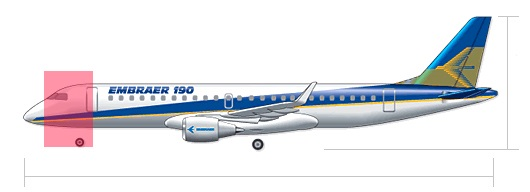
\includegraphics[scale=0.8]{images/ERJ190}
\caption{Posicionamento da LRU}
\label{fig:ERJ190}
\end{figure}


Foi selecionado um objeto sem texturas e com material brilhante como mostrado na
imagem~\ref{fig:LRU} por sofrer mais influ�ncia em varia��o de ilumina��o e ser
�nico na janela de inspe��o em quest�o.

\begin{figure}[h!]
\centering
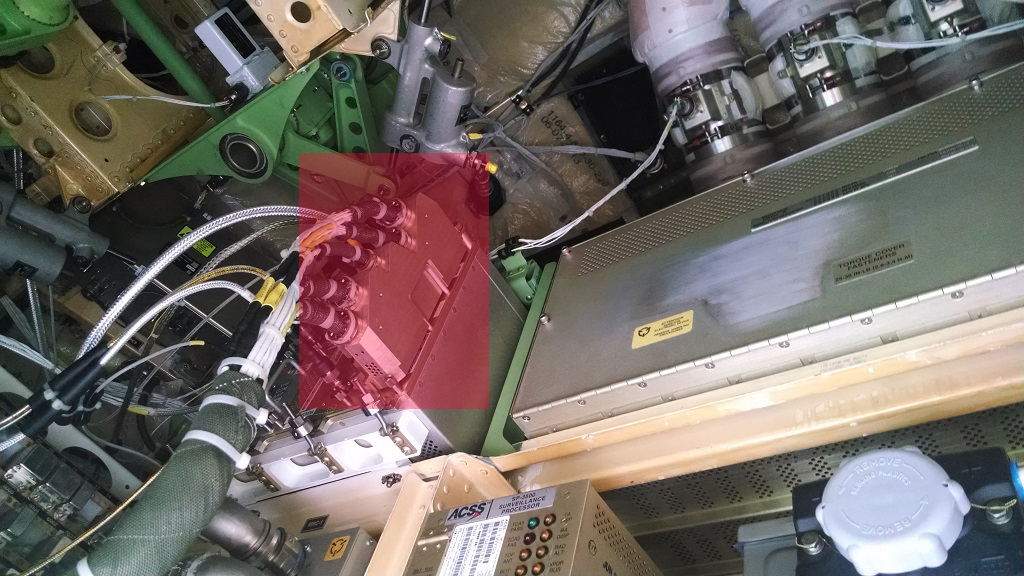
\includegraphics[scale=0.4]{images/LRU}
\caption{Imagem da LRU}
\label{fig:LRU}
\end{figure}

 


 \section{Caso de uso}
O presente trabalho tem como objetivo geral avaliar o ambiente de manuten��o aeron�utico interno, no contexto de janelas de inspe��o e tra�ar estrat�gias de reconhecimento de items de manuten��o.
Para a consecu��o do objetivo geral, foram definidos os seguintes objetivos espec�ficos:


\begin{itemize}
\item Avaliar as algoritmos cl�ssicos de reconhecimento;
\item Levantar caracter�sticas padr�o dos objetos no contexto;
\item Avaliar limites de percep��o humanas das caracter�sticas padr�o;
\item Avaliar algoritmo mais adequado para o contexto.
\end{itemize}
	
A proposta dessa tese � a partir do cen�rio de manuten��o de aeronaves e da proposta de utiliza��o de realidade aumentada, determinar a melhor estrat�gia de reconhecimento de pe�as para que posteriormente seja utilizado em ferramentas de auxilio na manuten��o por meio da realidade aumentada

\cite{ISMAR2012}
\cite{ORB}
\section{Fundamenta��o Te�rica}


\subsection[Realidade Aumentada]{Realidade Aumentada}
\begin{frame}
\frametitle{Realidade Aumentada}

A realidade aumentada � uma t�cnica de vis�o
computacional em que valendo-se de artefatos do mundo real, tem por objetivo
causar sensa��o de imers�o do usu�rio em um ambiente aumentado por artefatos virtuais, ao contr�rio de ambientes puramente virtuais 
como � comum em aplica��es de realidade virtual
\end{frame}

\begin{frame}
\frametitle{Realidade Aumentada Aplicada}


\begin{figure}[H]
\centering
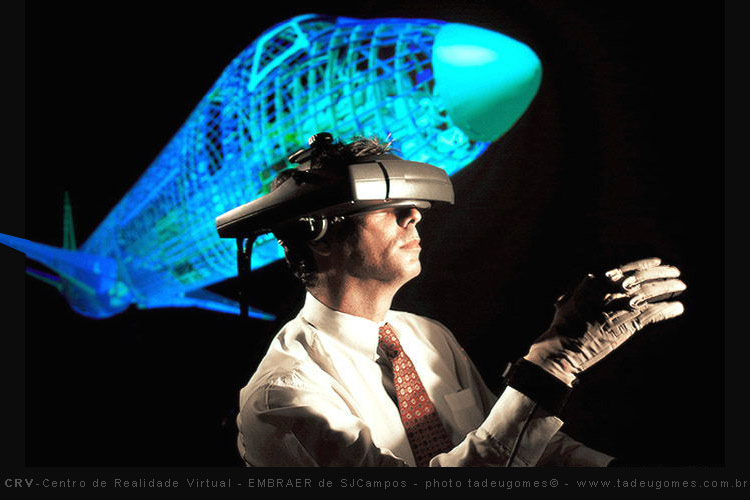
\includegraphics[scale=0.2]{images/realidade-virtual}
\caption{Ambiente Imersivo. Fonte CRV EMBRAER}
\label{fig:rv}
\end{figure}


\end{frame}


\begin{frame}
\frametitle{Realidade Aumentada Aplicada}


\begin{figure}[H]
\centering
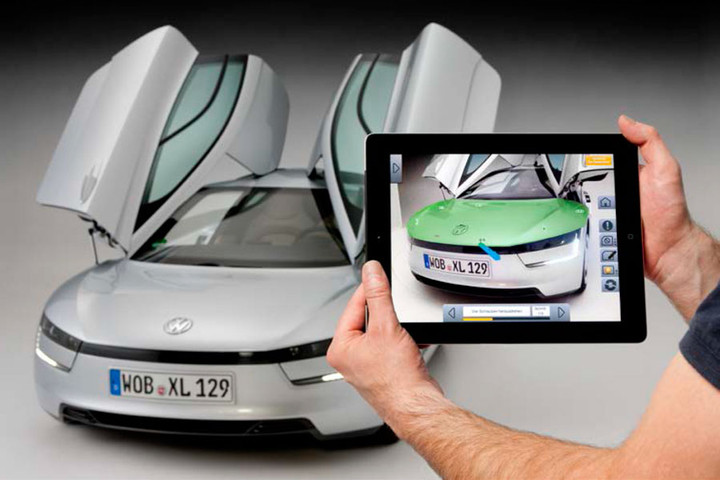
\includegraphics[scale=0.2]{images/ar}
\caption{Aplica��o de Realidade Aumentada no meio automobil�stico
Fonte www.metaio.com.br}
\label{fig:reconhecimento}
\end{figure}


\end{frame}




\begin{frame}

\frametitle{Processo de Realidade Aumentada}

\begin{figure}[H]
\centering
\begin{tikzpicture}[scale=0.9 ,transform shape]

  \node[draw,rectangle] (a) {Captura};
  \node[draw,rectangle,below of=a] (b) {Prepara��o};
  \node[draw,rectangle,below of=b] (c) {Detec��o};
  \node[draw,rectangle,below of=c] (d) {Reconhecimento};
  \node[draw,rectangle,below of=d] (e) {Rastreio};
  \node[draw,rectangle,below of=e] (f) {Apresenta��o};

  % 1st pass: draw arrows
  \draw[vecArrow] (a) to (b);
  \draw[vecArrow] (b) to (c);
  \draw[vecArrow] (c) to (d);
  \draw[vecArrow] (d) to (e);
  \draw[vecArrow] (e) to (f);
    
    
  % 2nd pass: copy all from 1st pass, and replace vecArrow with innerWhite
  \draw[innerWhite] (a) to (b);
  \draw[innerWhite] (b) to (c);
  \draw[innerWhite] (c) to (d);
  \draw[innerWhite] (d) to (e);
  \draw[innerWhite] (e) to (f);

  % Note: If you have no branches, the 2nd pass is not needed

\end{tikzpicture}
  \caption{Processo Can�nico de Realidade Aumentada}
  \label{diagram:pipelinera}

\end{figure}


\end{frame}


\subsection[Caracter�sticas]{Caracter�sticas}
\begin{frame}
\frametitle{Caracter�sticas}

\begin{figure}[H]
\centering
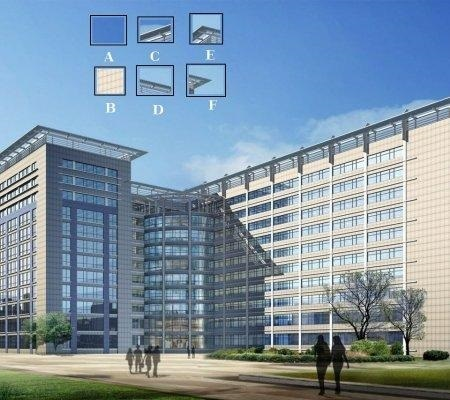
\includegraphics[scale=0.45]{images/features}
\caption{Reconhecendo caracter�sticas.
Fonte \cite{localfeaturedetector}}
\label{fig:reconhecimento}
\end{figure}


\end{frame}


\begin{frame}
\frametitle{Detector de caracter�stica}


\end{frame}


\begin{frame}
\frametitle{Descritor de caracter�stica}



\end{frame}







\section{Reconhecimento}

� a etapa em que padr�es s�o identificados e comparados para posteriormente identificar objetos

 
\begin{figure}[h!]
\centering
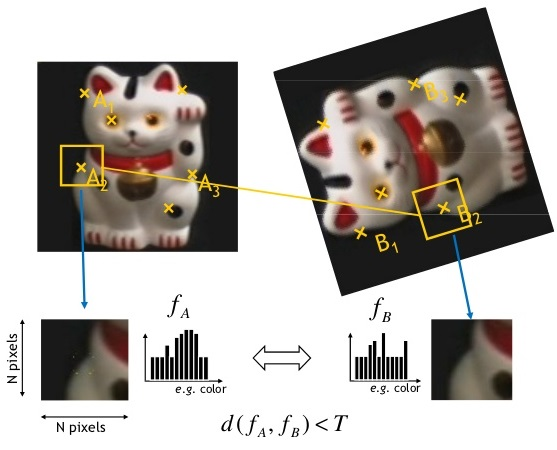
\includegraphics[scale=1.0]{images/reconhecimento}
\caption{Ilustra��o do procedimento de reconhecimento com features locais.}
\label{fig:reconhecimento}
\end{figure}

Pipeline de reconhecimento como ilustrado na imagem~\ref{fig:reconhecimento} :
\begin{itemize}
	\item Encontrar um grupo de keypoints distintos
	\item Definir uma regi�o em torno de cada keypoint 
	\item Extrair e normalizar o conte�do da regi�o
	\item Calcular um descritor para a regi�o normalizada
	\item Encontrar correspond�ncias de descritores.  
\end{itemize}


\section{Caracter�sticas Locais}
Caracter�sticas locais s�o padr�es em imagens que diferenciam padr�es de seu
vizinho imediato, sendo que as mais comuns s�o intensidade, cor e texturas.

\subsection{Caracter�sticas}
Antes de compreender como � feito o reconhecimento e registro de imagens � importante nos perguntar
 como n�s conseguimos reconhecer objetos em uma cena, como conseguimos comparar facilmente objetos em duas 
 imagens distintas. Somos treinados desde cedo a diferenciar formas geom�tricas, perceber escalas diferentes 
 ou mesmo reconhecer o mesmo objeto independente de como est� posicionado na cena buscando padr�es que 
 categorizem e diferenciem o objeto. Instintivamente conseguimos reconhecer boas caracter�sticas e localizar objetos.
Na Figura~\ref{fig:padroes} temos uma Figura de um pr�dio e seis recortes, dos quais
conseguimos facilmente reconhecer com precis�o a de letra E e F, as de letra A,B,C,D
 podemos identificar poss�veis localiza��es mas n�o podemos dizer com certeza onde est�o na Figura.

\begin{figure}[H]
\centering
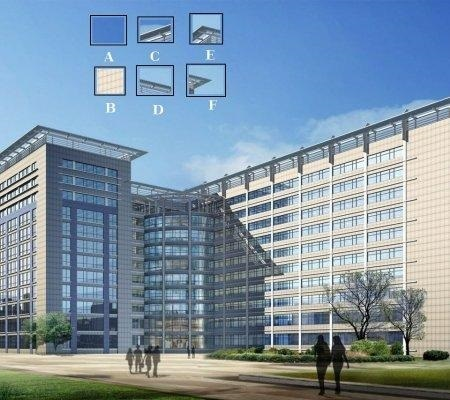
\includegraphics[scale=1.0]{images/features}
\caption{Reconhecimento de padr�es. Fonte \cite{understandingfeatures}}
\label{fig:padroes}
\end{figure}
As caracter�sticas E e F s�o o que consideramos boas caracter�sticas, pois o
n�vel de certeza � bem alto.

\begin{figure}[H]
\centering
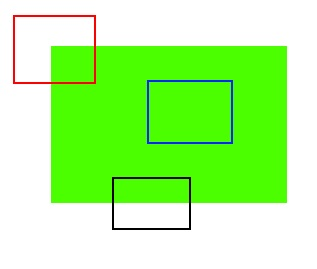
\includegraphics[scale=1.0]{images/featuresregioes}
\caption{Regi�es de reconhecimento de padr�es. Fonte
\cite{understandingfeatures}}
\label{fig:featuresregioes}
\end{figure}

A Imagem~\ref{fig:featuresregioes} ilustra tipos de caracter�sticas. A regi�o
azul n�o possibilita diferenciar onde est� na Figura, a regi�o preta pode ser confundida com qualquer uma das regi�es
 ao deslocarmos horizontalmente, a Figura vermelha nos possibilita diferenciar e reconhecer o canto da Figura verde 
 com precis�o milim�trica.
Podemos ent�o concluir que uma caracter�stica � boa para ser utilizada como par�metro de entrada
 para algoritmos de reconhecimento, quanto maior foi o n�vel de certeza da sua localiza��o, 
 o que facilita o \emph{\textbf{Feature Detection}}.
Para localizar o mesmo objeto em outra Figura � necess�rio identificarmos a regi�o onde se encontra, 
caso contr�rio no exemplo da Figura~\ref{fig:padroes} seria imposs�vel
localizar uma janela espec�fica. Tal descri��o de contexto � chamada de
\emph{\textbf{Feature Description}}. Uma vez de posse da caracter�stica e do seu
contexto � poss�vel reconhecer o objeto de fato.


\subsection{Propriedades da Caracter�stica Local ideal}
Algoritmos de reconhecimento baseam-se em compara��es de caracter�sticas
recuperadas da cena.
A recupera��o e compara��o de pontos tem um custo computacional relevante perto do tempo de execu��o 
da aplica��o, portanto selecionar o menor n�mero poss�vel de caracter�sticas aumenta o desempenho e diminui 
o tempo de resposta da aplica��o.
Garantir que  s�o selecionadas boas caracter�sticas pode ser
crucial na efic�cia do reconhecimento.
Segundo \cite{localfeaturedetector} , boas caracter�sticas devem ter as
seguintes propriedades:

\begin{itemize}
	\item \textbf{Repetibilidade}: Dadas duas imagens do mesmo objeto ou cena,
	tomadas em condi��es ou pontos de vista diferentes, uma porcentagem alta de caracter�sticas deve
	 ser reconhecida se estiverem vis�veis.
	\item \textbf{Distin��o}: Os padr�es reconhecidos t�m de ser poss�veis de serem
	distinguidos entre si para facilitar o casamento.
	\item \textbf{Localidade}: As caracter�sticas devem ser locais para reduzir a
	probabilidade de oclus�o.
	\item \textbf{Quantidade}: O n�mero de pontos detectados tem que ser o
	suficiente para que mesmo objetos pequenos tenham minimamente caracter�sticas que possam ser localizados e para que o 
	objeto possa sofrer oclus�o e ainda assim ser reconhecido.
	\item \textbf{Exatid�o}: As caracter�sticas detectadas tem que ser localizadas
	com o m�ximo de exatid�o poss�vel com respeito tanto referente � posi��o quanto
	� escala.
	\item \textbf{Efici�ncia}:De prefer�ncia  a detec��o deve ser o mais r�pido
	poss�vel.
\end{itemize}



\subsection{Detec��o de caracter�sticas}
O primeiro passo para o reconhecimento de objetos � a detec��o de caracter�sticas.Para que possa ser feita a compara��o da
 imagem referencia com a imagem sentida. A abstra��o de informa��es a ser reconhecida tem que ser suficiente para lidar 
 com escalas diferentes, rota��es entre as imagens, e pequenas distor��es.
Para que o reconhecimento seja eficiente e eficaz s�o necess�rios que uma massa de pontos m�nima seja selecionada e feita
 a correspond�ncia entre as imagens sentidas e refer�ncia.
As caracter�sticas utilizadas s�o em geral cantos, linhas, curvas, padr�es ou regi�es.
O tipo de caracter�stica selecionada � dependente do tipo de imagem provida. Imagens de cenas
 feitas a m�o geralmente s�o compostas de segmentos de retas enquanto imagens de sat�lite s�o geralmente compostas de 
 contornos e regi�es.
Quanto mais invariantes forem as caracter�sticas encontradas, mais robusto e preciso � o processo de compara��o.

\subsection{Correspond�ncia de caracter�sticas}
A fase de correspond�ncia de caracter�sticas � feita tanto selecionando caracter�sticas na imagem refer�ncia e procurando a 
correspondente na imagem sentida ou mesmo selecionando caracter�sticas nas duas imagens independentemente e procurando a 
correspond�ncia entre elas.
Quando a caracter�stica selecionada n�o for do tipo ponto, � importante para cada par de correspond�ncias, pelo menos uma 
ponto ser determinado para que seja utilizado para determinar posteriormente os par�metros de transforma��o. Por exemplo, 
se forem selecionados padr�es como tipo de caracter�stica, o centro do padr�o � considerado o ponto, se for selecionado 
uma regi�o, o centro de massa da regi�o � o ponto de apoio, se linhas forem tomadas como tipo de caracter�stica, devem 
ser tomados intersec��es como ponto de apoio e finalmente se forem selecionadas curvas, os m�ximos locais s�o considerados
 os pontos correspondentes.
 
 \section{Algoritmos de Reconhecimento}
\label{sec:algoritmos}
Existem diversos algoritmos de reconhecimento de caracter�sticas, entretanto
 nesse artigo os testes ser�o restritos aos algoritmos BRISK, FAST, FREAK, GFTT, MSER, ORB,
 STAR, SURF, SIFT.
Este cap�tulo se prop�e a dar uma vis�o geral dos algoritmos, pois o foco do
presente trabalho est� na an�lise comparativa entre os mesmos e n�o em cada um
dos algoritmos, visto exiistir implementa��es conceituadas no OpenCV, framework
utilizado.

%\input{parts/algoritmos/brief}

 \input{parts/algoritmos/fast}
 \input{parts/algoritmos/brisk}

 \input{parts/algoritmos/freak}
 \input{parts/algoritmos/gftt}
 \input{parts/algoritmos/mser}
 \input{parts/algoritmos/orb}
 \input{parts/algoritmos/sift}
 \input{parts/algoritmos/surf}
 \input{parts/algoritmos/star}







\section{Metodologia}
\subsection{Defini��o de par�metros}

Os testes ser�o realizados adicionando vari�veis de forma artificial por meio de transforma��es afins de forma a emular algum comportamento ou situa��o encontrada no ambiente de manuten��o
\begin{itemize}
	\item Varia��o de escala para simular a aproxima��o dentro da janela de
	inspe��o
	\item Varia��o de rota��o para simular a movimenta��o durante a manuten��o
	\item Varia��o de ilumina��o para simular manuten��es feitas em hor�rios do dia
	e ilumina��o diferente como por exemplo ambientes com neve com brilho muito maior
	\item Adi��o de \emph{Blur} para emular ambientes com muita poeira ou
	esfuma�ados
\end{itemize}

A defini��o das faixas de par�metro utilizados foi feita com inspe��o em campo

\section{An�lise de dados}
\label{sec:analisededados}

A an�lise de desempenho de cada t�cnica deve ser balizada por par�metros que garantam que a aplica��o seja vi�vel para o
 contexto citado na Se��o\ref{sec:restricao}. Para tal deve-se considerar os
 par�metros estimados abaixo definidos por inspe��o 

\begin{itemize}
	\item Cad�ncia > 5fps ou seja, tempo < 200ms \cite{Tang93whydo}
	\item Robustez � escala:  0.5 < escala < 1.2
	\item Robustez � rota��o:  0 < rota��o < 30 
	\item Robustez � ilumina��o: -50 < ilumina��o < 50
	\item Robustez � \emph{blur}: \emph{kernelsize} < 4
\end{itemize}

Uma an�lise mais precisa dos par�metros n�o faz parte do escopo desse trabalho
pois envolve pesquisa de campo em situa��es adversas. Portanto tais par�metros
foram escolhidos para validar o m�todo de sele��o das t�cnicas.




\cite{performance_evaluation}


Os algoritmos SIFT e SURF apesar de retornarem bons resultados para o contexto,
s�o pagos e portanto ser�o desconsiderados para a abordagem proposta.

Para que sejam respeitados as restri��es citadas na se��o~\ref{sec:restricao} e
para que a aplica��o seja coerente para uso cotidiano no contexto de manuten��o
de aeronaves, a velocidade de reconhecimento � muito importante. Uma an�lise
pr�via dos algoritmos selecionados tem como tempo de resposta por
frame a imagem~\ref{fig:performance6algorithms} que nos mostra claramente que as
t�cnicas MSER e FREAK n�o respondem em tempo �bil para serem considerados tempo
real, portanto ser�o desconsiderados.



\begin{figure}[h!]
\centering
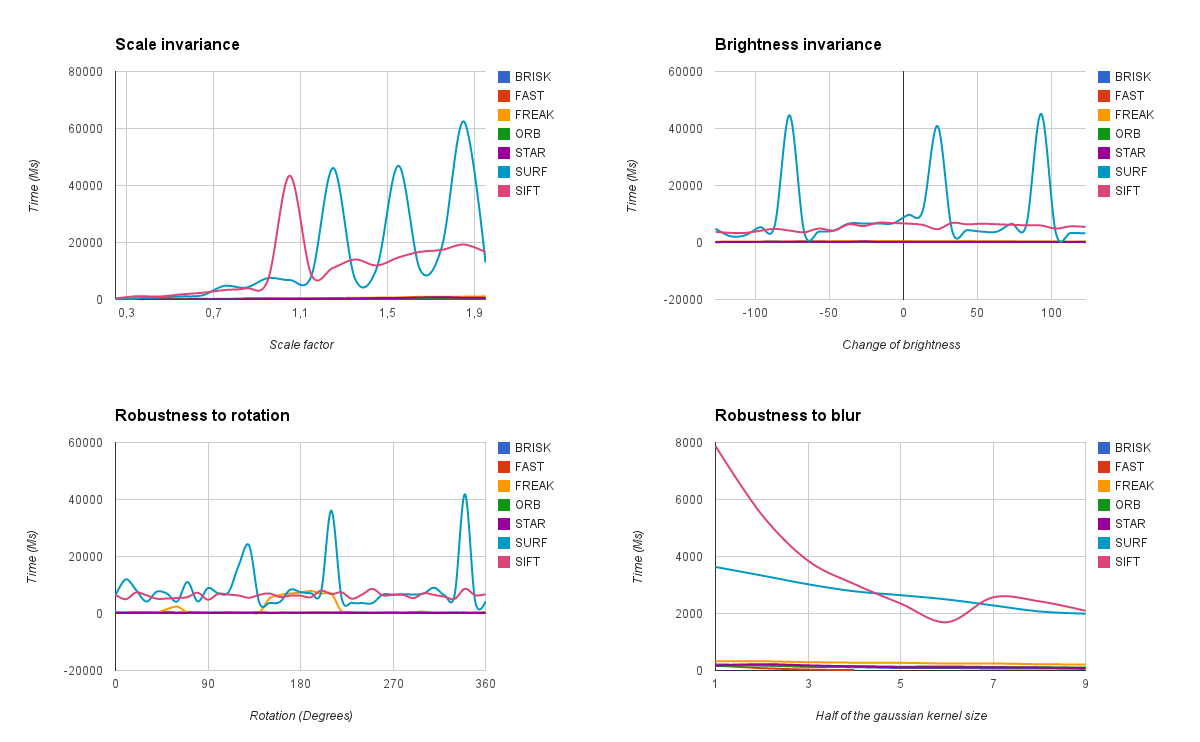
\includegraphics[scale=0.3]{images/time_sift_surf}
\caption{Performance quanto � varia��es de escala, ilumina��o, rota��o e
gaussian blur}
\label{fig:performance6algorithms}
\end{figure}


\begin{figure}[h!]
\centering
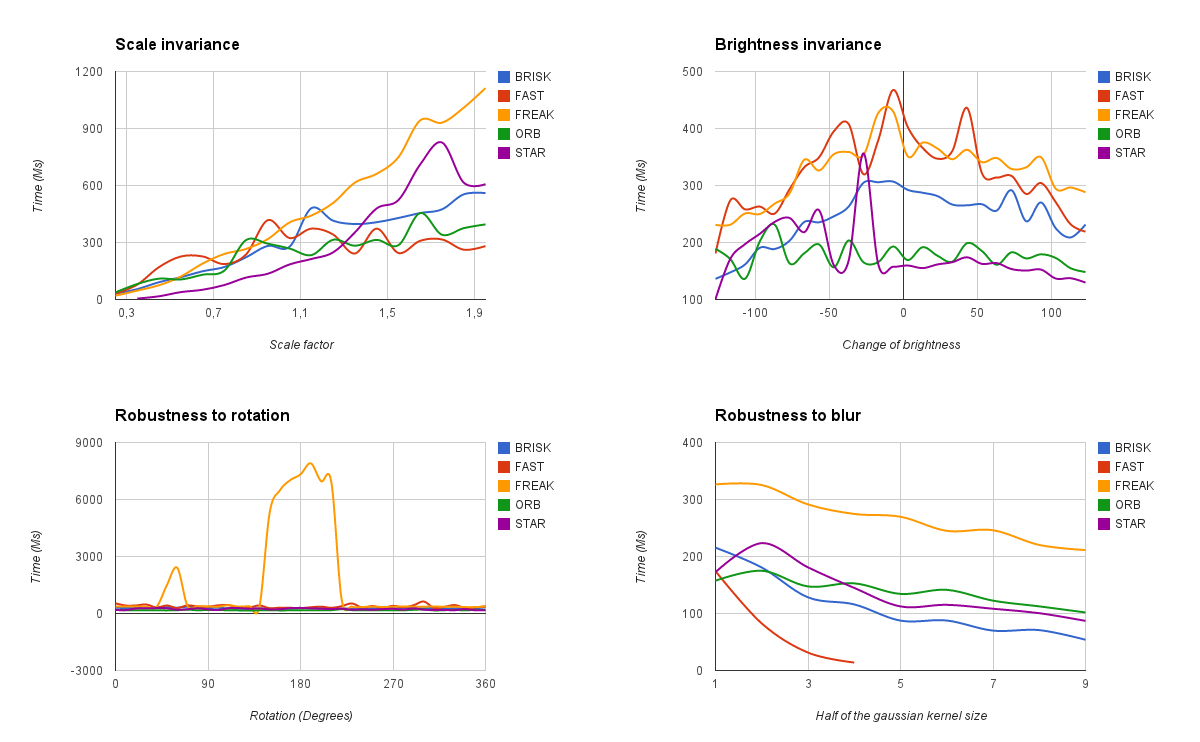
\includegraphics[scale=0.3]{images/time}
\caption{Performance quanto � varia��es de escala, ilumina��o, rota��o e
gaussian blur sem os algoritmos SIFT e SURF}
\label{fig:performance6algorithms}
\end{figure}



\section{Homografia}

Ap�s a etapa de extra��o de caracter�sticas da imagem padr�o e da imagem de
compara��o � importante fazer o casamento de padr�es para que com um n�mero
significativo de caracter�sticas, o objeto seja reconhecido. As imagens
imagem~\ref{fig:blurhomography}, mostram correspond�ncias entre imagens variando
as transforma��es propostas pelo prot�tipo em compara��o com imagens sem as
transforma��es.

\begin{figure}[h!]
\centering
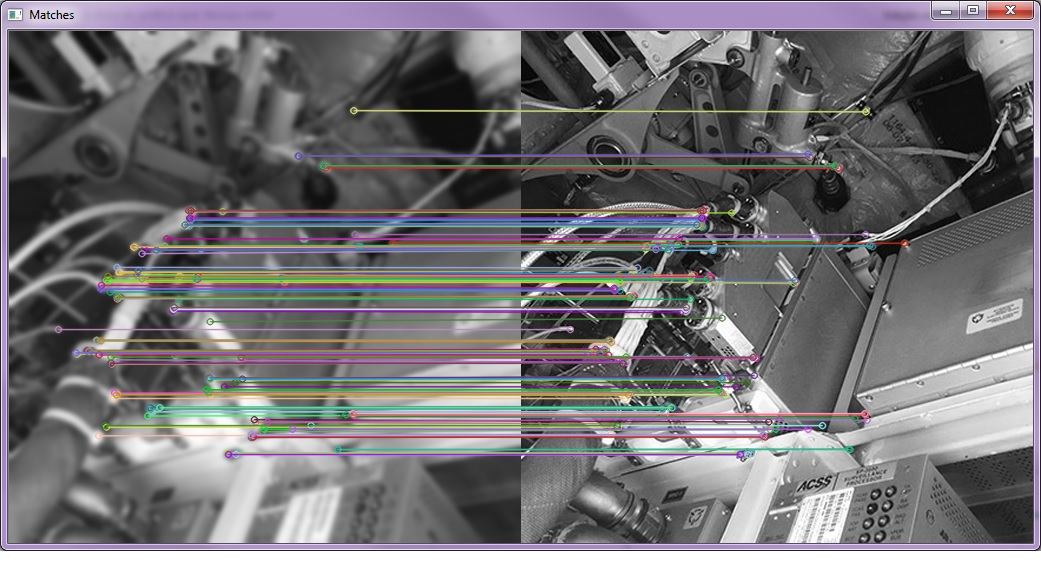
\includegraphics[scale=0.5]{images/ORB-BLUR-HOMOGRAPHY}
\caption{Homografia com varia��o varia��o de Blur.}
\label{fig:blurhomography}
\end{figure}

\begin{figure}[h!]
\centering
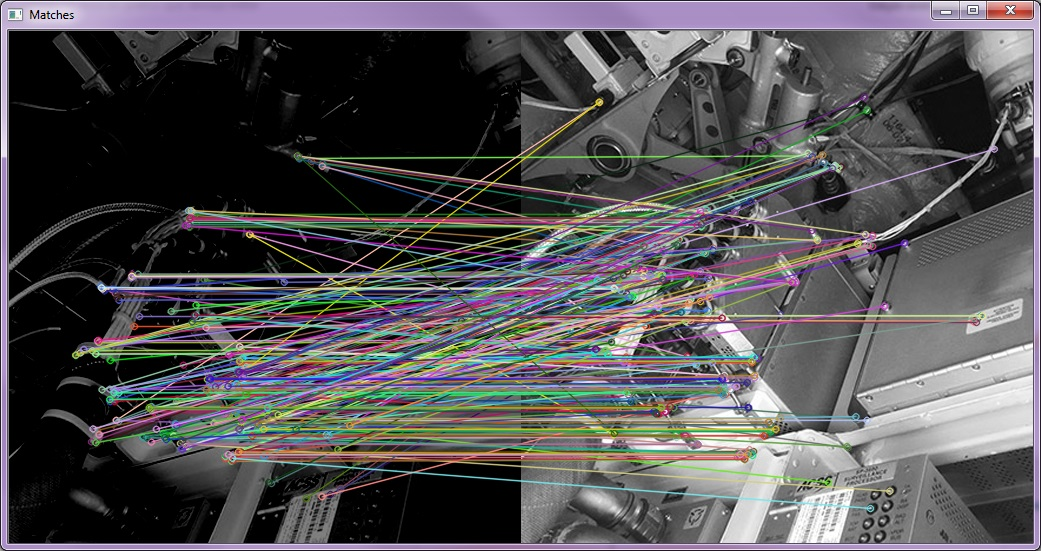
\includegraphics[scale=0.5]{images/ORB-BRIGHT-HOMOGRAPHY}
\caption{Homografia com varia��o varia��o de ilumina��o.}
\label{fig:brighthomography}
\end{figure}




\begin{figure}[h!]
\centering
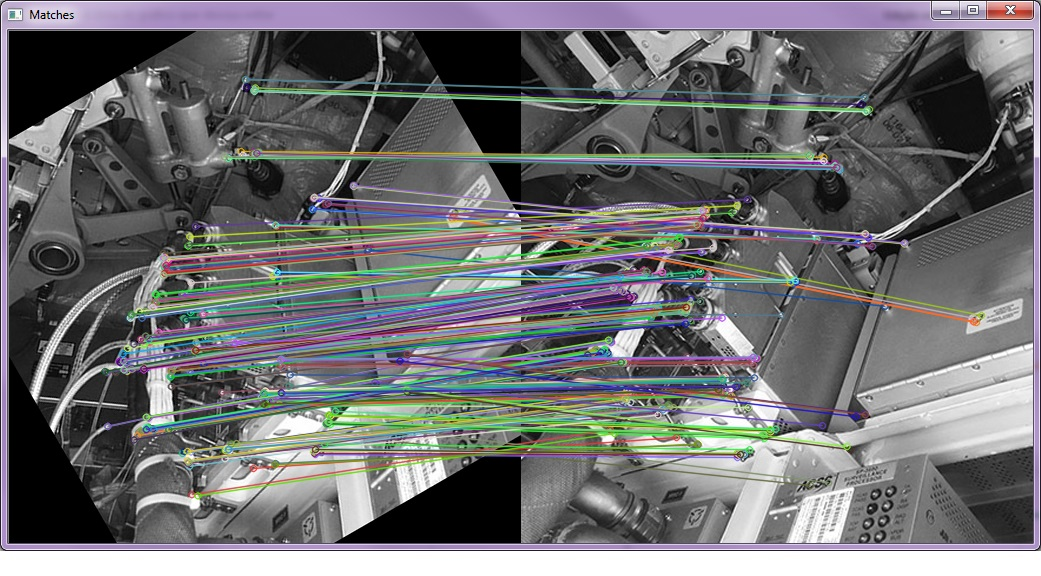
\includegraphics[scale=0.5]{images/ORB-ROTATION-HOMOGRAPHY}
\caption{Homografia com varia��o varia��o de Rota��o.}
\label{fig:rotationhomography}
\end{figure}



\begin{figure}[h!]
\centering
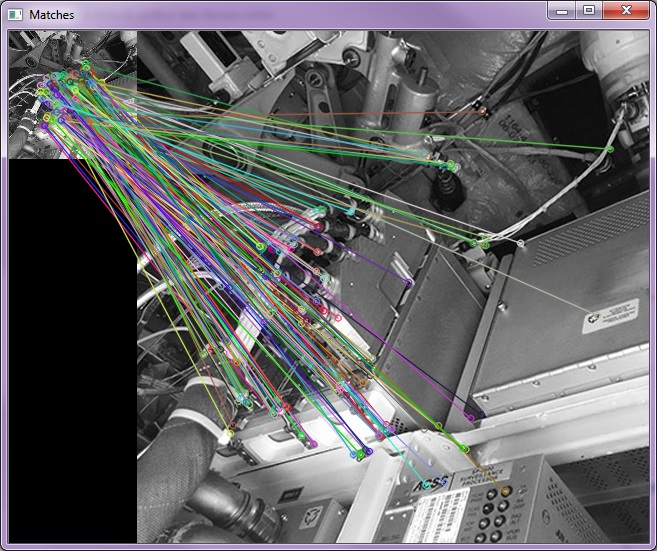
\includegraphics[scale=0.8]{images/ORB-SCALE-HOMOGRAPHY}
\caption{Homografia com varia��o varia��o de Escala.}
\label{fig:scalehomography}
\end{figure}



\cite{ISMAR2012}

Este trabalho apresentou uma metodologia de compara��o de algoritmos de
reconhecimento de padr�es tendo como caso de uso o contexto aeron�utico, mais
expecificamente no reconhecimento de pe�as do interior da aeronave, objeto de
manuten��o.
Os conceitos b�sicos de Realidade Aumentada e dos algoritmos utlizados foram
apresentados para fornecer meios ao conhecimento dessa tecnologia, que s�o
fundamentais para compreender melhor a proposta do trabalho.
Com o objetivo de tra�ar uma metodologia de decis�o imparcial foram descritos
algumas restri��es impostas � an�lise que posteriormente foram aplicados nos
resultados das simula��es.
Foram feitos testes emulando situa��es de varia��o ambiental pois fazer os
testes em ambientes e situa��es reais demandaria um custo muito elevado, al�m
dos resultados serem semelhantes.
Dessa forma concluiu-se que GFTT Se��o~\ref{sec:gftt}  e ORB Se��o~\ref{sec:orb}
s�o os mais favor�veis para o contexto proposto no trabalho.

\subsection{Atendimento dos objetivos}

\textbf {Avaliar as algoritmos cl�ssicos de reconhecimento}

O trabalho apresentou os algoritmos cl�ssicos na Se��o~\ref{sec:algoritmos},
descrevendo seu funcionamento e realizando testes de desempenho com os mesmos.


\textbf {Selecionar algoritmo mais adequado para o contexto}

Foi feita uma an�lise comparativa entre os algoritmos com as mesmas imagens de
teste e configurando o prot�tipo da mesma maneira, para que a �nica vari�vel no
momento fosse a t�cnica em quest�o.
Levantadas restri��es atrav�s de par�metros emp�ricos definidos por an�lise de
engenharia, com os valores mais prov�veis no contexto.
Para a sele��o das t�cnicas mais adequadas, foram utilizadas as restri��es e
criado nos gr�ficos, janelas de decis�o e gerado uma matriz de decis�o com os
resultados de todos os testes, tanto de qualidade de reconhecimento quanto de
tempo de execu��o.




\section{Trabalhos Futuros}

A utiliza��o de Realidade Aumentada no campo da manuten��o pode trazer muitos
ganhos no que tange � usabilidade levando ao usu�rio uma quantidade de informa��es que da maneira tradicional por meio inspe��o e consulta em manuais
seria invi�vel.
Este trabalho teve como foco o reconhecimento de padr�es em um cen�rio
aeron�utico espec�fico, como pr�ximos passos temos:
\begin{itemize}

\item Adequar a aplica��o para dispositivos m�veis como tablets, celulares ou
mesmo dispositivos HMD de forma a dar mais flexibilidade ao condutor da
manuten��o;

\item Realizar o casamento de padr�es com v�deos e imagens tempo real utilizando
as t�cnicas identificadas, otimizando a aplica��o para se tornar o mais tempo
real e aceit�vel poss�vel;

\item Adaptar a aplica��o para utilizar processamento paralelo e processamento
em GPU visto os algoritmos serem recursivos e localmente independentes.

\item Analisar por meio de testes em campo com poss�veis usu�rios para abstrair
par�metros de usabilidade como por exemplo determinar que tipo de informa��es
seriam �teis ao usu�rio ou mesmo que tipo de configura��o de dispositivo seria o
mais adequado para uma aplica��o desse porte.
\end{itemize}
\section{Agradecimento}

\begin{frame}


\huge
\textbf{Obrigado}

\large
Bruno Duarte Corr�a

\small
\color{blue}{bruno.duartec@gmail.com}


\end{frame}


\bibliography{bibliography}

\end{document}
